\twocolumn[
\begin{center}
\title{\color[cmyk]{1, 0.57, 0, 0.38}{\Huge\bfseries Creazione di RPM \\}} % definisco il titolo dell'articolo
\author{\scriptsize Gabriele Trombini(mailga@fedoraonline.it)} % definisco l'autore e altre informazioni
\date{}
\end{center}
{\color[cmyk]{1, 0.46, 0, 0}\LARGE (Parte prima) RPM - introduzione}\\
\maketitle
\normalsize
\doublespacing
\hfill
]
\definecolor{shadecolor}{cmyk}{0, 0, 0, 0.8}
\onehalfspacing
\lettrine[lines=1, loversize=0.1, lraise=0.1]{\color[cmyk]{0.5, 0, 1, 0}\bfseries c}{}on l'acronimo {\itshape rpm} (RedHat Package Manager) si identifica sia il formato dei pacchetti usati da Fedora che l'utility per la loro gestione.\\

A dire il vero, seppur nato da Red Hat, questo formato riscosse fin dall'inizio un grande successo (al pari del formato .deb usato da debian e derivate), tant'è che ancora oggi viene utilizzato da altre distribuzioni (come Mandriva e Opensuse, inizialmente derivate da Red Hat) per l'installazione degli applicativi.\\

Lo stesso Fedora Project ne ha adottato lo standard come riferimento.\\

Malgrado vi siano diversi tools (come alien o checkinstall, anche se quest'ultimo non ha avuto nuove versione dal 2009) che permettono la creazione di {\itshape rpm}, con questo articolo vogliamo seguire le specifiche del Fedora Project riguardanti la creazione di un pacchetto dal punto di vista di un collaboratore packager, così come specificato all'indirizzo {\itshape http://fedo\\raproject.org/wiki/ Packaging:Guidelines}, tralasciando quindi le modalità di gestione, manutenzione e ispezione dei pacchetti mediante l'utilizzo del comando rpm e relative opzioni\\

Le linee guida sono molto dettagliate ed è consigliabile seguirle analiticamente in modo particolare qualora si volesse contribuire al progetto o mantenere i pacchetti di Fedora.

\begin{center}
{\bfseries Preparazione}
\end{center}

Come prima cosa è indispensabile che gli strumenti necessari alla corretta esecuzione delle operazioni siano installati sul propro computer:

\begin{shaded}
{\color[cmyk]{0, 0, 0, 0}\# yum install @Strumenti$\backslash$ di$\backslash$ sviluppo}
\end{shaded}

\begin{shaded}
{\color[cmyk]{0, 0, 0, 0}\# yum install fedora-packager}
\end{shaded}

Quest'ultimo comando installa come dipendenza anche l'utility {\itshape rpmdevtools} che ci consente di utilizzare il comando adatto alla creazione dell'albero per lo sviluppo:

\begin{shaded}
{\color[cmyk]{0, 0, 0, 0}\$ rpmdev-setuptree}
\end{shaded}

Al termine del comando possiamo controllare che nella home dell'utente in uso sia presente la cartella rpmbuild, che a sua volta contiene altre directory (al momento vuote).

\begin{figure*}[!ht]
\centering
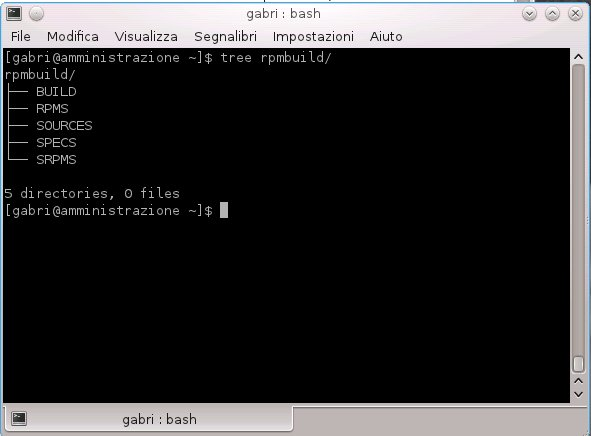
\includegraphics[scale=.95]{articoli/sistema_avanzato/immagini/rpmbuild_tree.jpeg}
\caption{l'albero di sviluppo dei pacchetti }
\end{figure*}

\begin{itemize}
\item SOURCES — dove devono essere inseriti i file sorgenti, le patch ed i file di icone;
\item SPECS — dove devono essere inseriti i file .spec;
\item BUILD — dove i sorgenti saranno scompattati ed il pacchetto costruito;
\item RPMS — dove il processo build inserirà il pacchetto binario;
\item SRPMS — dove il processo build inserirà il pacchetto sorgente.
\end{itemize}

A questo punto tutto è pronto per cominciare il nostro lavoro di packaging ma, se vogliamo essere conformi a quanto previsto dal Fedora Project, è bene che si legga in particolare le specifiche riguardanti:

\begin{enumerate}
\item nomenclatura ({\itshape http://fedoraproje\\ct.org/wiki/Packaging:NamingGui\\delines\ \#Package\_Naming\_and\_\\Versioning\_Guidelines});
\item versione e release ({\itshape http://fedora\\project.org/wiki/Packaging:Nami\\ngGuidelines\#Package\_Version});
\item aspetti legali ({\itshape https://fedoraproje\\ct.org/wiki/Packaging/Guidelines\#\\Legal});
\item licenza ({\itshape http://fedoraproject.org\\/wiki/Packaging:LicensingGuideli\\nes});
\end{enumerate}

Oltre a quanto sopra, occorre tenere presente anche altri aspetti, di carattere più pratico, legati alla preparazione dei pacchetti per la nostra distribuzione.\\
 
\begin{itemize}
\item tutto il software presente deve essere libero ed opensource;
\item le inclusioni devono essere inserite partendo dai sorgenti;
\item non costruire i pacchetti utilizzando l'utente root (è possibile creare un utente per lo sviluppo);
\item seguire le direttive di layout del FHS (Filesystem Hierarchy Standard) che definisce come devono essere distribuiti i file nel sistema e, se si dovesse avere necessità di creare nuove directory, è bene chiedere, motivando l'operazione, al Fedora Packaging Committee;
\item non inserire file in /bin, /sbin, /lib or /lib64, bensì utilizzare /usr/bin, /usr/sbin, /usr/lib, and /usr/lib64 (è possibile usare dei link simbolici a queste directory);
\end{itemize}

Come già detto Il Fedora Packaging Committee può rispondere ad eventuali dubbi.\\

\begin{figure}[!ht]
\centering
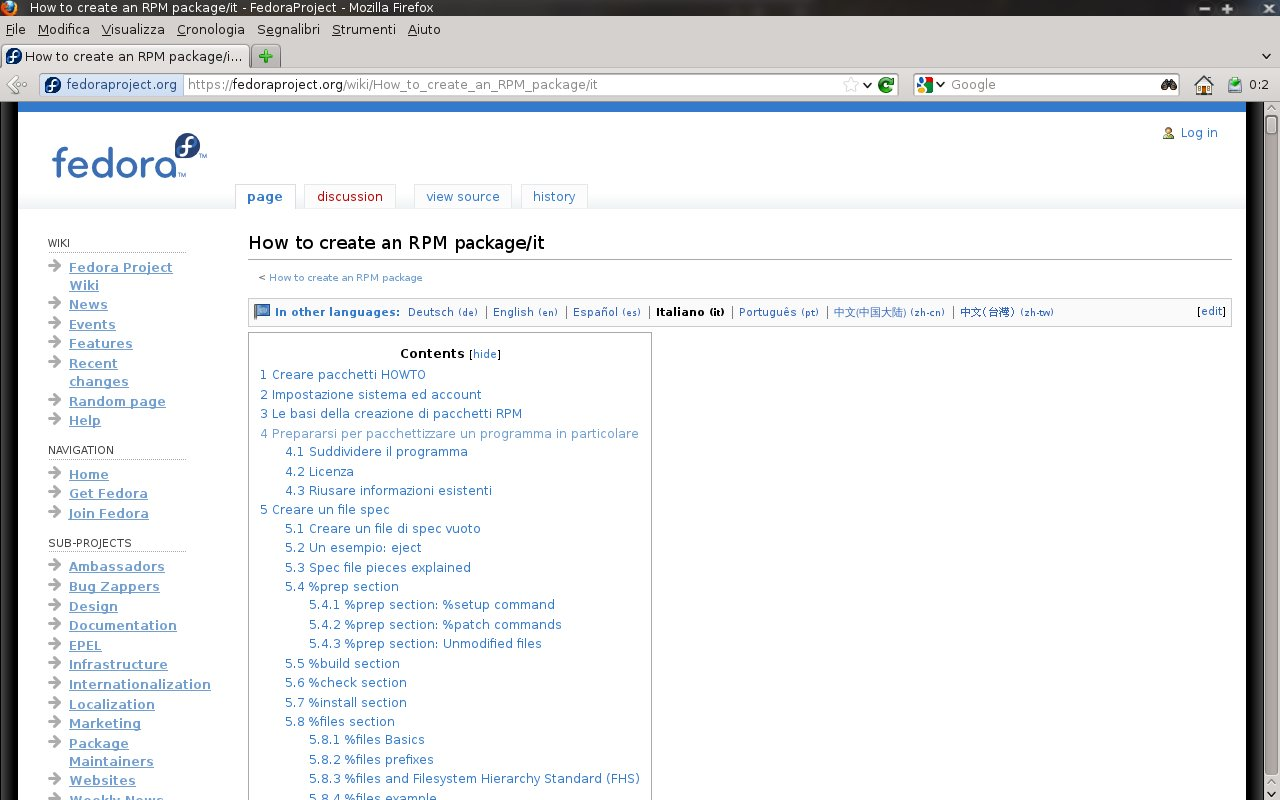
\includegraphics[scale=.21]{articoli/sistema_avanzato/immagini/rpm_wiki.jpeg}
\caption{come creare un rpm, la pagina tradotta dal team italiano}
\end{figure}

Arrivati a questo punto abbiamo preparato il nostro sistema per il packaging e siamo pronti ad eseguire il processo secondo le indicazioni del Progetto Fedora.\\

Il passo successivo che vedremo nel prossimo numero, sarà quello di creare il file {\itshape .spec}, un fondamentale file di testo contenente le informazioni necessarie alla pacchettizzazione dell'applicativo.\\


\hfill {\itshape (fine prima parte)}


\begin{comment}
Il primo passaggio da considerare è dato dal file .spec, un semplice file di testo contenente le informazioni necessarie alla pacchettizzazione dell'applicativo.

Fasi dell'rpmpbuild:

Nome della Macro 	Nome 	Di solito 	Scopo
%_specdir	directory della Specifica	~/rpmbuild/SPECS	file di specifica RPM (.spec)
%_sourcedir	directory Source	~/rpmbuild/SOURCES	Pacchetto dei sorgenti incontaminati (es: tarballs) e patch
%_builddir	Build directory	~/rpmbuild/BUILD	Source files are unpacked and compiled in a subdirectory underneath this.
%_buildrootdir	directory root di Build 	~/rpmbuild/BUILDROOT	I file vengono installati qui durante la fase %install.
%_rpmdir	directory dei binari RPM directory	~/rpmbuild/RPMS	Binari RPM sono creati e immagazzinati qui sotto.
%_srcrpmdir	directory dei Sorgenti RPM	~/rpmbuild/SRPMS	Il sorgente RPM sono creati e immagazzinati qui sotto. 

Creare un file spec

E' necessario creare ora il file ".spec" nella directory "~/rpmbuild/SPECS". E' consigliato dare al file il nome del programma, es: "programma.spec". Usa il nome dell'archivio oppure il nome sostenuto dall'autore del programma dove possibile, ma assicurati di rispettare le Linee guida per il Naming dei pacchetti.
Creare un file di spec vuoto

Quando crei uno spec file per la prima volta, è possibile usare la versione iniziale emacs o vim (dalla 7.1.270-1) che creano automaticamente un template per voi, ES.:

 $ cd ~/rpmbuild/SPECS
 $ vi program.spec

Di seguito un esempio di questo template:

Name:		
Version:	
Release:	1%{?dist}
Summary:	
Group:		
License:	
URL:		
Source0:	
BuildRoot:	%{_tmppath}/%{name}-%{version}-%{release}-root-%(%{__id_u} -n)

BuildRequires:	
Requires:	

%description

%prep
%setup -q

%build
%configure
make %{?_smp_mflags}

%install
rm -rf %{buildroot}
make install DESTDIR=%{buildroot}

%clean
rm -rf %{buildroot}

%files
%defattr(-,root,root,-)
%doc

%changelog


Puoi avere $RPM_BUILD_ROOT al posto di %{buildroot}; basta che sia consistente.

Puoi usare il comando rpmdev-newspec per creare un file di spec per te. rpmdev-newspec NOME-DEL-NUOVO-PACCHETTO crea un file spec iniziale per un nuovo pacchetto, su misura per vari tipi di pacchetti. Il programma individuerà il tipo di template da usare dal nome del pacchetto, o puoi specificare un particolare tipo di modello; controlla /etc/rpmdevtools/spectemplate-*.spec per consultare i template disponibili. Controlla rpmdev-newspec --help per maggiori informazioni. Per esempio, per creare un nuovo file di spec per un modulo python:

cd ~/rpmbuild/SPECS
rpmdev-newspec python-antigravity
vi python-antigravity.spec

Un esempio: eject

Di seguito un esempio, un pacchetto per Fedora 9 per il programma "eject":

Summary: A program that ejects removable media using software control
Name: eject
Version: 2.1.5
Release: 11%{dist}
License: GPL
Group: System Environment/Base
Source: http://metalab.unc.edu/pub/Linux/utils/disk-management/%{name}-%{version}.tar.gz
Source1: eject.pam
Patch1: eject-2.1.1-verbose.patch
Patch2: eject-timeout.patch
Patch3: eject-2.1.5-opendevice.patch
Patch4: eject-2.1.5-spaces.patch
Patch5: eject-2.1.5-lock.patch
Patch6: eject-2.1.5-umount.patch
BuildRoot: %{_tmppath}/%{name}-%{version}-%{release}-root
URL: http://www.pobox.com/~tranter
ExcludeArch: s390 s390x
BuildRequires: gettext
BuildRequires: automake
BuildRequires: autoconf
BuildRequires: libtool

%description
The eject program allows the user to eject removable media (typically
CD-ROMs, floppy disks or Iomega Jaz or Zip disks) using software
control. Eject can also control some multi-disk CD changers and even
some devices' auto-eject features.

Install eject if you'd like to eject removable media using software
control.

%prep
%setup -q -n %{name}
%patch1 -p1 -b .versbose
%patch2 -p1 -b .timeout
%patch3 -p0 -b .opendevice
%patch4 -p0 -b .spaces
%patch5 -p0 -b .lock
%patch6 -p1 -b .umount

%build
%configure
make

%install
rm -rf %{buildroot}

make DESTDIR=%{buildroot} install

# pam stuff
install -m 755 -d %{buildroot}/%{_sysconfdir}/pam.d
install -m 644 %{SOURCE1} %{buildroot}/%{_sysconfdir}/pam.d/%{name}
install -m 755 -d %{buildroot}/%{_sysconfdir}/security/console.apps/
echo "FALLBACK=true" > %{buildroot}/%{_sysconfdir}/security/console.apps/%{name}

install -m 755 -d %{buildroot}/%{_sbindir}
pushd %{buildroot}/%{_bindir}
mv eject ../sbin
ln -s consolehelper eject
popd

%find_lang %{name}

%clean
rm -rf %{buildroot}

%files -f %{name}.lang
%defattr(-,root,root)
%doc README TODO COPYING ChangeLog
%attr(644,root,root) %{_sysconfdir}/security/console.apps/*
%attr(644,root,root) %{_sysconfdir}/pam.d/*
%{_bindir}/*
%{_sbindir}/*
%{_mandir}/man1/*

%changelog
* Wed Apr 02 2008 Zdenek Prikryl <zprikryl at, redhat.com> 2.1.5-11
- Added check if device is hotpluggable
- Resolves #438610



    Name: The (base) name of the package. It must follow the Package Naming Guidelines. In many cases, this will be in all lower case. Elsewhere in the spec file, you can refer to the name using the macro %{name} - that way, if the name changes, the new name will be used by those other locations. This name should match the spec file name.
    Version: The upstream version number. See Packaging/Naming guidelines - package version for more information. If the version is non-numeric (contains tags that are not numbers or digits), you may need to include the additional non-numeric characters in the release field. If upstream uses full dates to distinguish versions, consider using version numbers of the form yy.mm[dd] (so a 2008-05-01 release becomes 8.05). Elsewhere in the spec file, refer to this value as %{version}.
    Release: The initial value of the release should normally be "1%{?dist}". Then, increment the number every time you release a new package for the same version of software. If a new version of the software being packaged is released, the version number should be changed to reflect the new software version, and the release number should be reset to 1. See Name Guidelines - package release for more. Packaging/DistTag describes the "dist" tag, which isn't required but can be useful. Use %{release} to reuse this value.
    Summary: A brief, one-line summary of the package. Use American English, and do not end in a period.
    Group: This needs to be a pre-existing group, like "Applications/Engineering"; run "less /usr/share/doc/rpm-*/GROUPS" to see the complete list. If you create a sub-package "...-doc" with documentation, use the group "Documentation".
    License: Its license; for software, this must be an open source software license. Use a standard abbreviation, e.g., "GPLv2+". Try to be specific, e.g., use "GPLv2+" (GPL version 2 or greater) instead of just "GPL" or "GPLv2" where it's true. See Licensing and the Licensing Guidelines for more information. You can list multiple licenses by combining them with "and" and "or", e.g., "GPLv2 and BSD". Call this tag "License"; don't use the older, inaccurately named tag "Copyright".
    URL: The URL for more information about the program, e.g., the project website. Note: This is NOT where the original source code came from, see "Source" (next!).
    Source0: The URL for the compressed archive containing (original) pristine source code, as upstream released it. "Source" is synonymous with "Source0". If you give a full URL (and you should), its basename will be used when looking in the SOURCES directory. If possible, embed %{name} and %{version}, so that changes to either will go to the right place. Warning: Source0: and URL: are different - normally they are both URLs, but the "URL:" entry points to the project website, while the "Source0:" entry points to the actual file containing the source code (and is typically a .tar.gz file). As noted in the guidelines, "When downloading sources, patches etc, consider using a client that preserves the upstream timestamps. For example wget -N or curl -R. To make the change global for wget, add this to your ~/.wgetrc: timestamping = on, and for curl, add to your ~/.curlrc: -R." If there is more than one source, name them Source1, Source2, and so on. If you're adding whole new files in addition to the pristine sources, you can list each of them as sources as well, but list them after the pristine sources. A copy of each of these sources will be included in any source package you create (unless you specially direct otherwise). See Packaging/SourceURL for more information on special cases (using revision control, when upstream uses prohibited code, etc.).
    Patch0: The name of the first patch that you will apply to the source code. If you need to patch the files after they've been uncompressed, you should edit the files, save their differences as a "patch" file in your ~/rpmbuild/SOURCES directory. Patches should make only one logical change, so it's quite possible to have multiple patch files.
    BuildArch: If you're packaging files that are architecture-independent (e.g., shell scripts, data files, etc.), then add "BuildArch: noarch". The architecture for the binary RPM will then be "noarch".
    BuildRoot: This is where files will be "installed" during the "%install" process (which happens after the %build compilation process). Normally you should just leave this line alone; under the usual Fedora setup, this will be a macro that will create a new special directory under /var/tmp. Newer versions of RPM will ignore this value, and instead place the build root in "%{_topdir}/BUILDROOT/".
    BuildRequires: A comma-separated list of packages required for building (compiling) the program. These are not automatically determined, so you need to include everything needed to build the program. There are a few packages that are so common in builds that you don't need to mention them, such as "gcc"; see the Packaging Guidelines for the complete list of the packages you may omit. You can also specify minimum versions, if necessary, like this: "ocaml >= 3.08". You can have more than one line of BuildRequires (in which case they are all required for building). If you need file /EGGS, you can get its package by running "rpm -qf /EGGS"; if EGGS is a program, you determine its package quickly by running "rpm -qf `which EGGS`". Try to specify only the minimal set of packages necessary to properly build the package, since each one will slow down a "mock"-based build (e.g., try to use sed instead of perl if you don't really need perl's abilities). Watch out: Some applications permanently disable functions if their package isn't detected during the build; in those cases you may need to include those additional packages. If you have trouble figuring out this list, the "auto-br-rpmbuild" command (from the auto-buildrequires package) may be helpful.
    Requires: A comma-separate list of packages that are required when the program is installed. Note that the list of packages for Requires (what's required when installing/running) and BuildRequires (what's required to build the binary RPM) are independent; a package may be in one list but not the other, or it could be in both. The dependencies of binary packages are in many cases automatically detected by rpmbuild, so it is often the case that you don't need to specify the Requires tag at all. But if you want to highlight some specific packages as being required, or require a package that rpm can't detect should be required, then add it here.
     %description - A longer, multi-line description of the program. Use American English. All lines must be 80 characters or less. "Blank lines are assumed to separate paragraphs. Some graphical user interface installation programs will reformat paragraphs... (lines that) start with whitespace, such as a space or tab, will be treated as preformatted text and displayed as is, normally with a fixed-width font." (per the RPM Guide).
     %prep - Script commands to "prepare" the program, that is, to uncompress it so that it will be ready for building (compiling). Typically this is just "%setup -q" or some variation of it; a common variation is "%setup -q -n NAME" if the source file unpacks into NAME. See the "%prep" section below for more.
     %build - Script commands to "build" the program, that is, to compile it and get it ready for installing. The program should come with instructions on how to do this. See the "%build" section below for more.
     %check - Script commands to self-test the program. This is run after %build and before %install, so you should place it there if you have this section. Often it simply contains "make test" or "make check". This is separated from %build so that people can skip the self-test if they desire. This isn't documented in many places.
     %install - Script commands to "install" the program. The commands should copy the files from the "build directory" %{_builddir} (which would be under ~/rpmbuild/BUILD) into the buildroot directory, %{buildroot} (which would normally be under /var/tmp). See the "%install" section below for more.
     %clean - instructions to clean out the build root. Typically: 

rm -rf %{buildroot}

     %files - the list of files that will be installed. See the "%files" section below for more.
     %changelog - Changes in the package. Use the format example above.
    ExcludeArch: If the package does not successfully compile, build or work on an architecture, then those architectures should be listed in the spec in an ExcludeArch tag.
    You can add sections so that code will run when packages are installed or removed on the real system (as opposed to just running the %install script, which only does a pseudo-install to the build root). These are called "scriptlets", and they are usually used to update the running system with information from the package. See the "Scriptlets" section below for more. 

Don't use the tags "Packager" or "Vendor". Don't use "Copyright" - use "License" instead. Don't create a "relocatable" package - they don't add value in Fedora yet they make things more complicated.

RPM supports subpackages, that is, a single spec file can generate many binary packages. For example, if the documentation is very large, you might generate a separate "-doc" subpackage. See below for more.
 %prep section

The "%prep" section describes how to unpack the compressed packages so that they can be built. Typically, this is a set of "%setup" and/or %patch commands, which reference the Source0:, Source1:, etc. lines above. See the Maximum RPM section on %setup and %patch for more details.

Warning: In spec files, don't use in-line comments (a "#" comment on the same line after a command), and don't put macros (words beginning with "%") in a comment unless you quote the "%" as "%%". Macros can cause failures if they are in a comment, because they are always expanded (even when in a comment) and they can expand to multiple lines. This is true for %prep, %build, and so on.

The new RPM 4.4.2.x series adds two new macros, %{patches} and %{sources}, so you can do things like:

for p in %{patches}; do
...
done

These new macros can be very useful if you have a large list of patches or sources. However, keep in mind that using these will make your spec incompatible with the rpm used in Fedora 9 and earlier, RHEL, and many other RPM-based distros.
 %prep section: %setup command

The "%setup" command unpacks a source package, and takes several switches. Normally you should use "-q" (quiet) to prevent setup from babbling about every file it unpacks. Here are a few switches besides -q:

    -n name: If the name of the rpm is something other than what the Source unpacks to, use this switch to state the name it unpacks to. E.G., if the tarball unpacks into a directory MYNAME, use %setup -q -n MYNAME
    -c name: If the tarball doesn't unpack into a single directory, this creates a directory named name and then unpacks into it. Useful if you have one of those annoying tarballs that doesn't have a single common subdirectory embedded in it. 

There are more %spec options if you are unpacking multiple files, which is primarily useful if you are creating subpackages (see below). The key ones are:
-a number 	Only unpack the source directive of the given number, such as –a 0 for source0:, after changing to the directory.
-b number 	Only unpack the source directive of the given number, such as –b 0 for source0:, before changing to the directory.
-D 	Do not delete the directory before unpacking.
-T 	Disable the automatic unpacking of the archives.
 %prep section: %patch commands

The "%patch0" command applies patch 0 (similar for 1, 2, etc.). Patches are the normal way to change to the source code if necessary to package it. The normal "-pNUMBER" option applies, which simply passes that argument on to patch.

Patch file names often look like "telnet-0.17-env.patch", that is, %{name}-%{version}-patch_purpose.patch (some people omit -%{version}). Patch files are typically the result of a "diff -u"; if you do this from the subdirectory of ~/rpmbuild/BUILD, you won't have to specify a -p level later. You can use all the normal ways of creating a patch file.

If you're creating a patch file a single file FILENAME, a common way is to copy it to FILENAME.orig, modify it, and then save the results of "diff -u FILENAME.orig FILENAME". If you change directory to "~/rpmbuild/BUILD/NAME", you could create a patch file to change a single file by doing:

cp X/Y.Z X/Y.Z.orig
vim X/Y.Z
diff -u X/Y.Z.orig X/Y.Z > ~/rpmbuild/SOURCES/PKGNAME.REASON.patch

If you're going to edit many files, one easy method is to copy the whole subdirectory underneath BUILD, and then do subdirectory diffs; once you change directory to "~rpmbuild/BUILD/NAME", you can:

cp -pr ./ ../PACKAGENAME.orig/
... many edits ...
diff -u ../PACKAGENAME.orig . > ~/rpmbuild/SOURCES/NAME.REASON.patch

If you edit many files in one patch, you can also copy the original files using some consistent ending such as ".orig" before editing them. Then, you can use "gendiff" (in the rpm package) to create a patch with the differences. Do "man gendiff" for more information.

Try to ensure that in your patch the "context" matches exactly. In old versions of Fedora, the default "fuzz" value was 2, which meant that imprecise matches were acceptable. However, the version of RPM used by Fedora 10 and later have a default fuzz to 0, requiring that matches be exact. You can work around this by adding "%global _default_patch_fuzz 2", but it's better to not have the problem by making the patch match the context exactly.

As explained in Packaging/PatchUpstreamStatus, all patches in Fedora spec files SHOULD have a comment above them about their upstream status. This should document the upstream bug/email that includes it (including the date), or if it's Fedora-unique, why it is unique. The Fedora Project focuses, as much as possible, on not deviating from upstream in the software it includes in the repository - see Staying close to upstream projects for more about why it's important to do this.
 %prep section: Unmodified files

Sometimes, you'll package just a straight file that doesn't need to be uncompressed, e.g., a "Source1:" that is just a simple PDF file. These might not be from external sources, e.g., perhaps you've had to create a few additional files that weren't in the original sources so that the package cleanly installs in Fedora. You can "prep" those into the build directory by doing this (replace "1" with whatever number it is):

 cp -p %SOURCE1 .

 %build section

The "%build" section is sometimes complicated; here you configure and compile/build the files to be installed.

Many programs follow the GNU configure approach (or some variation). By default, they will install to a prefix of "/usr/local" (/usr/local/bin, /usr/local/lib, etc.), which is a reasonable default for unpackaged files. However, since you are packaging it, you will want to change the prefix to "/usr", since this is now a package maintained by the system itself. If there are any libraries, they'll need to be installed in the right directory, which is either /usr/lib or /usr/lib64 depending on the architecture (the actual value is in %{_libdir}).

Since the GNU "configure" system is so common, rpm pre-defines a macro named "%configure", which invokes GNU configure with the right options (e.g., it changes --prefix to /usr). This means that some variation of this will often work as a build command:

 %configure
 make %{?_smp_mflags}

Sometimes you'll want to override the variables of a makefile; you can easily do that by passing them as parameters to make, like this:

make %{?_smp_mflags} CFLAGS="%{optflags}" BINDIR=%{_bindir}

If you need to do something complicated with GNU-generated configure, take a look at "GNU autoconf, automake, and libtool". A good presentation on these as well as "make" is "Open Source Development Tools: An Introduction to Make, Configure, Automake, Autoconf" by Stefan Hundhammer.

Some programs use Cmake. See Packaging/cmake for some suggestions.

If you include some self-tests (and that's a good idea), put them in a separate "%check" section that immediately follows the "%build" area, instead of including them in %build. That way, it will be easy for the system to skip unnecessary self-tests.
 %check section

The "%check" section does testing, often it's "make test". This is not documented in many other sources of RPM info.
 %install section

The "%install" section is a set of script commands to "install" the program. The commands in this section should copy the files from a directory inside the "build directory" %{_builddir} (normally ~/rpmbuild/BUILD/something) into the build root directory, %{buildroot} (normally /var/tmp/something), creating the directories inside %{buildroot} as necessary.

Watch out: Some of the terminology is very misleading:

    The build directory (under which compilations occur during %build) and the build root (where files are copied into during the %install process) are different. The point of the %install process is to copy files, such as those under the build directory, to the right place in the build root. Perhaps "buildroot" should be called "installroot", but it's too late now, the terminology is entrenched.
    The build directory is normally ~/rpmbuild/BUILD, while the build root (where files get installed to during %install) is normally ~/rpmbuild/BUILDROOT. The %prep stage will normally create a subdirectory underneath the build directory as part of %setup, and populate the build directory with files (based on the source information in %_sourcedir, which is typically in ~/rpmbuild/SOURCES). During %build, the current directory will actually start at %{buildsubdir}, that newly-created subdirectory under the build directory. Typically %{buildsubdir} is something like ~/rpmbuild/BUILD/%{name}-%{version}.
    The "%install" script is not used when the binary rpm package is installed by the end-user!! The term "%install" is misleading, in fact, the script must not install the programs in the REAL final locations (e.g., in /usr/bin), but under the buildroot %{buildroot}. 

Normally, the install script would first erase the %{buildroot} directory, and then do some variation of "make install" (ideally using DESTDIR=%{buildroot}, if the program supports it). Here's an example of an %install section:

%install
rm -rf %{buildroot}
make DESTDIR=%{buildroot} INSTALL="install -p" CP="cp -p" install

Ideally, every program would have a "make install" command that supported the DESTDIR convention. If the program includes a "make install" that supports DESTDIR, where possible, use it. The DESTDIR convention supports redirecting file installations to descend from a specific directory, which is exactly what we want during %install.

Installing a program that does not support DESTDIR can be much harder, and no option is as good as native DESTDIR support. Consider these alternatives:

    Patch the makefile so that it does support DESTDIR. Create directories inside DESTDIR where necessary (feel free to use "mkdir -p", the "-p" option of mkdir is now standard and widely supported). Be sure to submit the patch upstream.
    Use "%makeinstall". Many older RPM documents suggest using "%makeinstall", which might work if "make install" doesn't support DESTDIR. However, as noted in the Fedora guidelines, the %makeinstall macro "must NOT be used when make install DESTDIR=%{buildroot} works. %makeinstall is (merely) a kludge that can work with Makefiles that don't make use of the DESTDIR variable...". Unfortunately, this sometimes has subtle failures, which is why %makeinstall should not be used if DESTDIR works. The reason is based on how %makeinstall works. The "%makeinstall" macro expands to something like "make prefix=%{buildroot}%{_prefix} bindir=%{buildroot}%{_bindir} ... install". Many programs will quietly recompile or change parts of the program when values like prefix are changed, resulting in an incorrect installation. See the Fedora guidelines if you want the details on why this approach can fail. You will probably need to create appropriate directories inside %buildroot before calling %makeinstall (e.g., mkdir -p %{buildroot}%{_bindir}/).
    Consider using the auto-destdir package. This requires "BuildRequires: auto-destdir", and changing "make install" to "make-redir DESTDIR=%{buildroot} install". This only works well if the installation uses only certain common commands to install files, like cp and install; see "man make-redir" for details.
    Do the installation "by hand", that is, instead of invoking a build system, copy the files to the correct locations. Basically, this would be a sequence that would create directories that weren't already created by the "BuildRequires" packages (typically using install -d or mkdir -p), followed by copying of files from the current directory (inside the build directory) into the buildroot directory (typically using "cp -p" and/or "install -p"). Running "make -n install" may make it easy to determine what this sequence should be. Be sure to create directories inside %buildroot where necessary. One serious problem with this approach is that it's easy to fail to install new or renamed files during an update—so if there's a better approach, use it instead. If you do perform the installation "by hand", be especially careful with updates when using this approach. For example: 

%install
rm -rf %{buildroot}
mkdir -p %{buildroot}%{_bindir}/
cp -p mycommand %{buildroot}%{_bindir}/

As noted in the packaging guidelines' timestamp section, "when adding file copying commands in the spec file, consider using a command that preserves the files' timestamps, eg. cp -p or install -p". So, if the makefile lets you override the install command (typically named INSTALL), you might want something like INSTALL="install -p" CP="cp -p" as make parameters, like this:

make INSTALL="install -p" CP="cp -p" DESTDIR=%{buildroot} install

 %files section

The %files section identifies what files and directories were added by the package - and thus, which files and directories are owned by the package. Ownership is important - when you type "rpm -qif blah", you'll see who owns blah. This section is used when performing the bin stage, to determine which files are placed into each binary RPM file.
 %files Basics

The %files section normally begins with a %defattr line which sets the default file permissions. The format of this is %defattr(<file permissions>, <user>, <group>, <directory permissions>), that is, one can specify the permissions to apply to files and directories in the %files section. The fourth parameter is often omitted. Usually one uses %defattr(-,root,root,-), where "-" means "use the default permissions".

This is followed by names or patterns of the directories or files to be installed and owned by this package. You should use macros for directory names, e.g., use %{_bindir}/myfile instead of /usr/bin/myfile, and %{_sbindir}/killaccount instead of /usr/sbin/killaccount. If a name or pattern begins with "/" when expanded, then it is presumed to have been copied into the %{buildroot} followed by that pattern; when installed on the final system, it will be copied into that name without the buildroot prefix. If you don't precede the pattern with "/", then it is presumed to be in the current directory (e.g., inside the build directory) - this is used for "documentation" files. So if your package just installs /usr/sbin/mycommand, then your %files section could simply say:

%files
%defattr(-,root,root,-)
%{_sbindir}/mycommand

Any file or directory identified in the %files section is owned by the defining package. You should make sure that you declare ownership of every new file or directory the package creates. You can use wildcards (*) which match a set of files - this makes the package less sensitive to changes. For example, you can declare that all the files that were copied into %{buildroot}/usr/bin are owned by this package by declaring:

%{_bindir}/*

Note that "%{_bindir}/*" does not claim that this package owns the /usr/bin directory - it claims that all the files that were installed inside the build root 's /usr/bin are owned by the package. If you list a directory in the %files section, then you are claiming that this package owns that subdirectory and all files and directories in it, recursively (all the way down) if they are present in the build root. Do not list the "/usr/bin" or "%{_bindir}" directories directly in your %files list, because that would claim ownership of /usr/bin and everything inside it. Claiming ownership of "%{_bindir}/*" is fine, though; that just claims ownership of the subdirectories and files you placed under %{buildroot}/%{_bindir}. If you create a subdirectory such as %{_datadir}/%{name}, (/usr/share/NAME), you should include that directory in the %files list:

%{_datadir}/%{name}/

It's usually easier to use wildcards for filenames, and that's also better at coping with changes in upstream. Older RPM documentation typically shows long lists under %files with individual names, such as /usr/bin/program1 followed by /usr/bin/program2. Because of the way Fedora now uses buildroots, that is no longer necessary.

It's an error if no file matches the wildcard of a line, so only note the directories that actually matter. Also, you can't identify the same file or directory more than once. Finally, it's an error to have something in the buildroot and not listed under %files; the whole point of copying something into the buildroot is because you intend to have it installed in the final system. If you don't intend that, remove those files during the %install process.

It is also possible to exclude files from a previous match by using a %exclude glob. This can be useful for including "almost all" of the files that match a different glob. However, note that, like any other file glob, even a %exclude glob will fail if it matches nothing. (This might be considered counterintuitive, as the whole point is essentially to ensure that a certain file ISN'T there, so this rule is especially important to remember.)
 %files prefixes

You may need to add one or more prefixes to a %files entry (if more than one, use a space to separate them).

Typically there is a "%doc" entry with a list of documentation files that didn't get copied into the buildroot; usually there is at least a README and LICENSE file. You must include the license file, if there is one. You may prefix some of these with %attr(mode, user, group) to set the file permission mode, user, or group. You don't need to claim ownership of the /usr/share/doc/%{name} directory, that's automatic if there's a %doc entry. Any %doc entry must not affect the runtime of the application (if it is in %doc, the program must run properly if it is not present).

There is a potential 'gotcha' with %doc entries: if you have a %doc entry, then you can't use commands during %install to copy files into the documentation directory descending from %_defaultdocdir. That's because if there's a %doc entry, rpmbuild will automatically remove the docdir files created by %install before installing the files listed with %doc. This can hit you if, for example, you want an "examples" subdirectory in the documentation directory. In this case, don't use "%doc" to mark documentation. Instead, create the directories and copy the files into %{buildroot}%{_defaultdocdir}/%{name}-%{version}/ during %install, and make sure that %files includes an entry for "%{_defaultdocdir}/%{name}-%{version}/". They will still be correctly marked as documentation.

If you save configuration files (under /etc - don't put them under /usr), you should normally prefix them with %config(noreplace) unless this program version uses a non-backwards-compatible configuration format (in which case, prefix them with %config).

Prefixing a %files entry with "%attr(mode, user, group)" lets you set the permissions for particular file(s), e.g., "%attr(0644, root, root)". A "-" means "use the default".

If a file is in particular natural language, use %lang to note that. E.G.:

%lang(de) %{_datadir}/locale/de/LC_MESSAGES/tcsh*

Programs using Locale files should follow the recommended method of handling the i18n files:

    find the filenames in the %install step:  %find_lang ${name}
    add the required build dependencies: BuildRequires: gettext
    use the found filenames: %files -f ${name}.lang 

Some documentation claims that %license and %readme are valid prefixes; they are not valid in Fedora. Use %doc instead.
 %files and Filesystem Hierarchy Standard (FHS)

You should follow the Filesystem Hierarchy Standard (FHS), i.e., ordinary application executables go into /usr/bin, global configuration files go into /etc, ordinary libraries go into /usr/lib, and so on, with one exception: executables that should not normally be executed directly by users or administrators should go into a subdirectory of /usr/libexec; usually you'd refer to the necessary directory as "%{_libexecdir}/%{name}".

You shouldn't be installing files under /usr/local; that is where unpackaged files go. Typically there will be a "prefix" attribute that lets you set the prefix to be "/usr" instead of "/usr/local".

Unfortunately, many programs' "normal" installation routines do not follow the FHS. In particular, many programs normally place architecture-independent libraries under /usr/lib, instead of under /usr/share as the FHS requires. The FHS /usr/lib section says that /usr/lib is for architecture-dependent data (e.g., ELF files like .so files), while /usr/share is for architecture-independent data. That way, systems with different CPUs can share /usr/share. There are many exceptions to this rule in Fedora (e.g., Python and Perl), but Fedora applies this rule more strictly than some distributions. Note, for example, that rpmlint will complain if you put just about anything other than ELF files into /usr/lib.
 %files example

Here's a simple example of a %files section:

%files
%defattr(-,root,root,-)
%doc README LICENSE
%{_bindir}/*
%{_sbindir}/*
%{_datadir}/%{name}/

Finding duplicates

The Fedora guidelines require that "A Fedora package must not list a file more than once in the spec file's %files listings."

You can list any duplicates of two binary packages by doing:

cd ~/rpmbuild/RPMS/ARCH # Substitute "ARCH" for your architecture
rpm -qlp PACKAGE1.*.rpm | sort > ,1
rpm -qlp PACKAGE2.*.rpm | sort > ,2
comm -12 ,1 ,2




Other tags

We noted the "Requires" and "BuildRequires" tags earlier. There are a few other tags for controlling dependencies: Provides, Obsoletes, Conflicts, and BuildConflicts.

    "Provides:" lets you list virtual package names that this package provides. Sometimes there are several different packages that can provide a function, and using packages won't care which one. In that case, each of the packages that provide the function should "provide" a virtual package, and then using packages can list the virtual package name under "Requires:". For example, several different packages might provide "latex"; if you depend on the virtual package "tex(latex)", then users can choose which package to get "latex" from. If you provide virtual packages, you might also want to use the "alternatives" system, but be careful: "alternatives" settings are system-wide, so if multiple users on the same system might want different defaults, don't use the alternatives system. You can find out what a given package provides (both virtual and non-virtual names) by querying "rpm -q --provides PACKAGENAME". Some virtual packages in Fedora are:
        MTA : Used for mail transport agents, such as sendmail.
        tex(latex) : Used for latex 
    "Obsoletes:" lets you state that installing this package should (normally) cause the removal of the other named package(s). This is useful when a package's name changes, or when a package wholly replaces a different package.
    "Conflicts:" lets you state what packages cannot be installed simultaneously this one. Obviously, try to avoid this if you can; see Packaging/Conflicts if you think you need to use it.
    "BuildConflicts:" lets you state what packages cannot be installed when building this package. Obviously, try to avoid this if you can. 

You can control which architectures a package builds (or doesn't build). For example, if your package can't compile on ppc, you can do this:

ExcludeArch: ppc

There's also an "ExclusiveArch" tag. The valid architectures one can specify in these tags are listed in the Architectures section.
Subpackages

A spec file can define more than one binary package, e.g., client and server, or runtime and developer packages. If there's a large amount of documentation, it may be split into a NAME-doc subpackage. You will always have one spec file and one source RPM (SRPM), even if there are multiple binary RPMs that they generate. A spec file that produces multiple binary packages still has only one creation process, so there is only one %prep, %build, %check, and %install section that creates all the files for all the packages.

In a spec file, use the %package directive to start defining a subpackage:

%package sub_package_name

By default, the subpackage name is PACKAGE_NAME, "-", SUBPACKAGE_NAME; you can use "-n" to override this and make a new name:

%package -n new_sub_package_name

After the %package directive, list the tags for the subpackage. This should include at least the "Summary:" and "Group:" tags and directives "%description SUBPACKAGE_NAME" and "%files SUBPACKAGE_NAME". Anything not specified by the subpackage will be inherited from its parent. For the directives, if you used "-n" with %package, you'll need it again for these directives. You need to specify the name for the other directives, e.g., %pre and %post, if you use them in the subpackage.

See the RPM Guide section on subpackages for more information.
Conditionals

You can insert conditional statements. E.G., you can test if you are creating a binary for a certain architecture with:

%ifarch ARCHITECTURE_NAME

the negated version with:

%ifnarch ARCHITECTURE_NAME

or the more general conditional:

%if TRUE_OR_FALSE

There is an optional "%else" section; all of these are closed with "%endif".
Application Specific Guidelines

There are many application-specific guidelines that can help you (e.g., for specific programming languages, applications, libraries, and build systems). Many of them are listed as part of the Application Specific Guidelines of Packaging/Guidelines. Examples of application-specific guidelines are those for:

    Cmake
    Emacs 

Failing that, some other ways of finding application-specific help are:

    The 'SEARCH' command on Fedoraproject.org.
    PackagingDrafts
    A Special Interest Group (SIG)
    Wiki pages prefixed with 'Packaging' 

Miscellaneous hints

Try to write your scripts so that when upstream makes changes, the packaging is likely to work when you change the version number and reload the source file(s). For example, if it contains *.txt files with execute bits, instead of doing:

 chmod a-x Filename1.txt Filename2.txt Filename3.txt

consider doing this, which will handle new filenames that use the same file naming convention:

 chmod a-x *.txt

If you want to see lots of examples of scriptlets, you can show all the scriptlets on installed programs using:

 rpm -qa --queryformat "\n\nPACKAGE: %{name}\n" --scripts | less

Packaging/FrequentlyMadeMistakes has information on frequently-made mistakes.

Don't try to interact with the user; RPM is designed to support batch installs. If an application needs to show a EULA, that needs to be part of its initial execution, not its installation.

You might not want to start services, because in a big install that could slow things down. If you install an init script, consider using chkconfig to arrange for the service to be started and stopped on the next reboot. Before uninstalling you should normally try to stop its services if it's running.

Uninstall should reverse most changes made during installation, but don't remove any user-created files.

Normally, if there are binary executables, a separate "debug" package is created with the symbols, and the symbols are stripped from the normal binary packages. If this shouldn't happen, you can disable the package-creation and stripping with:

%global _enable_debug_package 0
%global debug_package %{nil}
%global __os_install_post /usr/lib/rpm/brp-compress %{nil}

To prevent stripping you may also need to do this in the %install section:

export DONT_STRIP=1

A way to check for the version of Fedora in a spec file for conditional builds is:

%if 0%{?fedora} <= <version>

(The ? causes the macro to evaluate to blank if %fedora is not defined, and this causes the end result to be "0", which is a number and thus ok, while not interfering with the result if there is actually a value for %fedora.)

Note that the previous trick DOES NOT work in Koji "scratch" builds - %fedora is set during the creation of a source RPM. (Thus, this trick does work in actual Koji builds as the system extracts sources from the source RPM and rebuilds the source RPM with the appropriate %fedora value.)

There are also some recommendations and controversial tricks on PackageMaintainers/Packaging Tricks.

GUI programs must have a desktop entry (so that people can invoke it from a graphical menu). The Fedora packaging guidelines discuss desktop files. See also the desktop entry spec (for .desktop files) and icon theme spec (for icon-related materials such as those in /usr/share/icon).


http://tldp.org/HOWTO/RPM-HOWTO/
http://fedoraproject.org/wiki/How_to_create_an_RPM_package
http://www.faqs.org/docs/securing/chap3sec20.html
http://docs.fedoraproject.org/en-US/Fedora_Draft_Documentation/0.1/html/RPM_Guide/
http://fedoraproject.org/wiki/Packaging:Guidelines
http://fedoraproject.org/wiki/Tools/RPM/it
http://www.g-loaded.eu/2006/04/05/how-to-build-rpm-packages-on-fedora/
http://foster-johnson.com/rpm.html
http://www.rpm.org/max-rpm/index.html
http://docs.fedoraproject.org/en-US/Fedora_Draft_Documentation/0.1/html/RPM_Guide/ch-creating-rpms.html
https://fedoraproject.org/wiki/How_to_create_an_RPM_package/it
http://fedoraproject.org/wiki/Packaging:Guidelines


\end{comment}
